\documentclass{standalone}
\usepackage{tikz}
\usetikzlibrary{calc, shapes, patterns}

\begin{document}
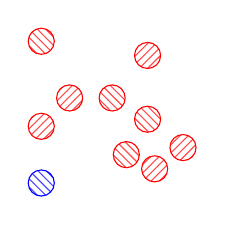
\begin{tikzpicture}[scale=.9]
	\node (A1) at (-1, -1) [circle, pattern=north west lines, pattern
        color=blue!70, draw=blue] {};
	\node (A2) at (-1, 1) [circle, pattern=north west lines, pattern
        color=red!70, draw=red] {};
	\node (A3) at (0, .2) [circle, pattern=north west lines, pattern
        color=red!70, draw=red] {};
	\node (A4) at (.2, -.6) [circle, pattern=north west lines, pattern
        color=red!70, draw=red] {};
	\node (A5) at (.5, -0.1) [circle, pattern=north west lines, pattern
        color=red!70, draw=red] {};
	\node (B1) at (-1, -.2) [circle, pattern=north east lines, pattern
        color=red!70, draw=red] {};
	\node (B2) at (1, -.5) [circle, pattern=north east lines, pattern
        color=red!70, draw=red] {};
	\node (B3) at (.5, .8) [circle, pattern=north east lines, pattern
        color=red!70, draw=red] {};
	\node (B4) at (-.6, .2) [circle, pattern=north east lines, pattern
        color=red!70, draw=red] {};
	\node (B5) at (.6, -.8) [circle, pattern=north east lines, pattern
        color=red!70, draw=red] {};
\end{tikzpicture}
\end{document}
